%----------------------------------------------------------------
%
%  File    :  state_of_the_art.tex
%
%  Authors :  David Lechner, FH Campus Wien, Austria
%
%  Created :  10 Oct 2019
%
%  Changed :  10 Oct 2019
%
%----------------------------------------------------------------


\chapter{Grundlagen}
\label{chap:state_of_the_art}

In diesem Kapitel werden die Grundlagen für das zu realisierende System beschrieben. Es beinhaltet eine Einführung in \textit{Machine Learning} und gibt dabei einen Überblick auf die verschiedenen Methoden und Anwendungsfälle. Zudem wird der \textit{Controller-Area-Network}-Bus vorgestellt, welcher für die Datensammlung im Kontext der Masterarbeit essenziell ist.
% TODO: Embedded-Systems?

\section{Machine Learning}
\label{sec:machine_learning}

\textit{Machine Learning} ist ein Bereich der Computer Wissenschaften und beschäftigt sich mit Algorithmen und Techniken zur Lösung von komplexen Problemen, wo konventionellen Programmiermethoden nicht vielversprechend sind. Wir werden heutzutage im alltäglichen Leben mit vielen Anwendungen konfrontiert, die ohne ML nicht möglich wären. Beispiele dafür sind Sprachsteuerung, Bild-, Gesichts- und Handschrifterkennung, Stauvorhersage aber auch Autonomes Fahren und die Erkennung von Brustkrebs \cite{KOUROU20158}. Schon vor 1980 wurde versucht einige solcher komplexen Probleme zu lösen, was jedoch nicht immer von Erfolg gekrönt war. Erst mitte der 2000er Jahre ist der Fortschritt in dem Bereich drastisch gestiegen. Gründe dafür gibt es mehrere. Zum einen ist mit dem Aufkommen des Internets eine viel größere Anzahl an Daten vorhanden und zum anderen sind Rechenleistung beziehungsweise Speicherplatz billiger, leichter zugänglich und vorallem performanter. Des Weiteren sind die Algorithmen verbessert und angepasst worden.
% TODO: auf Seite referenzieren?

Oft werden \textit{Machine Learning} und Künstliche Intelligenz (engl. \textit{Artificial Intelligence}, kurz AI) mit einander gleichgesetzt, was jedoch nicht stimmt. AI ist ein viel breitgefächerter Forschungsbereich, der mittels mehreren Ansätzen versucht Maschinen das "Denken" beizubringen. ML hingegen ist ein möglicher Ansatz dafür.

Um das Vorgehen zum Lösen eines komplexen Problems mittels \textit{Machine Learning} besser verstehen zu können, wird es im folgenden anhand einer Anwendung, welche handgeschrieben Buchstaben erkennt, erklärt. Zu aller erst wird eine Vielzahl an verschiedenen Datenpunkten (engl. \textit{data points}) - Bilder mit handgeschrieben Buchstaben - benötigt. Zusätzlich müssen diese mit dem enthaltenen Buchstaben markiert (engl. \textit{labelled}) sein. Das Ziel ist, dass die Anwendung nicht nur die Buchstaben im Datenset erkennt, sondern auch jene, die nicht enthalten sind. Mit der konventionellen Methode wird anfangs versucht zu verstehen wie die Bilder mit den Buchstaben zusammenhängen. Danach wird eine Reihe an Regeln festgelegt, um auch neue Bilder erkennen zu können. Da es jedoch eine große Variation von Handschriften gibt, kann das Regelset sehr schnell sehr groß werden. \textit{Machine Learning} Algorithmen gehen hierbei einen mehr generellen Lösungsweg, indem sie direkt von den markierten Daten lernen und sich das Regelset (engl. \textit{model}) selbst aneignen. Je mehr Bilder von Buchstaben vorhanden sind, desto genauer wird das ML-\textit{Model}. Werden neue Bilder ohne Markierung hinzugefügt, kann das \textit{Model} den Buchstaben erkennen. Diese Art um das Problem zu Lösen wird im Kontext von ML als Klassifizierung bezeichnet. Es gibt auch noch zwei weitere, welche adressiert werden:
\begin{itemize}
  \item Prognose (engl. \textit{Prediction}): Trainieren eines \textit{Models} mit historischen Daten zur Vorhersage zukünftiger Werte. Z.B. der Bedarf eines bestimmten Produktes in den Sommerferien.
  \item Klassifizierung (engl. \textit{Classification}): Datenpunkte in eine oder mehrere Kategorien bzw. Klassen einteilen. Z.B. Identifizierung einer Email als Spam oder nicht, Erkennen welches Tier auf einem Bild zu sehen ist (Katze, Hund, Löwe, \dots)
  \item Gruppierung (engl. \textit{Clustering}): Unterteilung vieler Datenpunkte in wenige Gruppen, in denen Punkte mit gleichen Eigenschaften enthalten sind. Im Gegensatz zur Klassifizierung ist die Anzahl der Gruppen im vorhinein nicht bekannt.
\end{itemize}

Zur besseren Vorstellung veranschaulicht Abbildung \ref{fig:ml_problem_types} die Arten. Abschnitt \ref{sec:ml_regression} und folgende gehen darauf näher ein.

\begin{figure}[htbp]
	\centering
		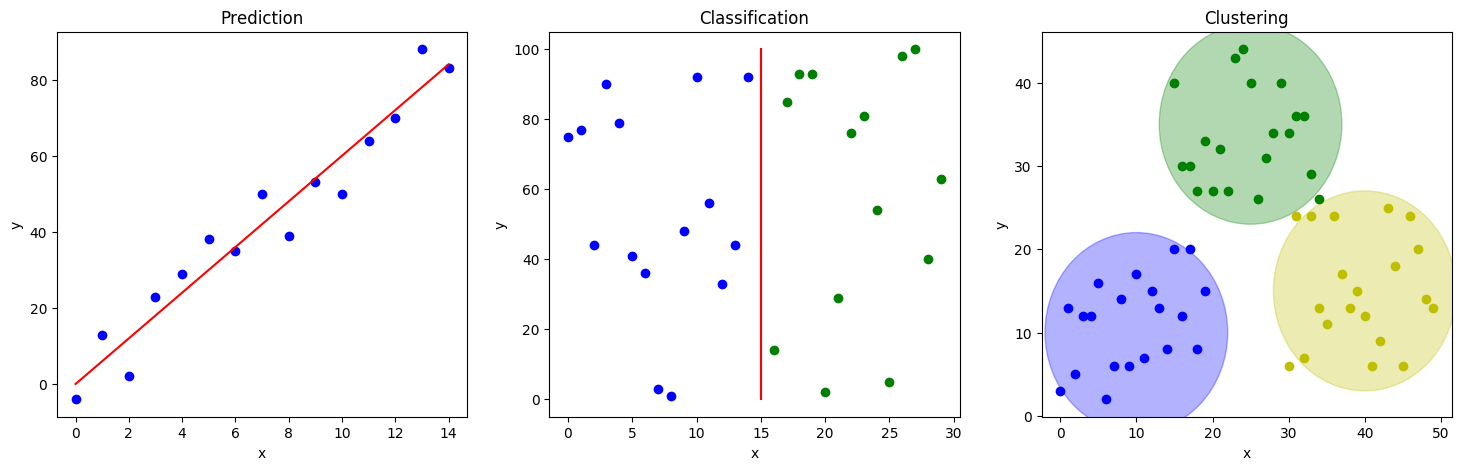
\includegraphics[width=\textwidth]{images/ml_problem_types.png}
	\caption{Arten von \textit{Machine Learning} Problemen (Quelle: Author)}
	\label{fig:ml_problem_types}
\end{figure}


\subsection{Ansätze}
\label{sec:ml_types}

Um ein ML-\textit{Model} anzulernen gibt es verschiedene Möglichkeiten. An eine davon - das Überwachte Lernen - wurde bereits in der Einführung anhand eines Beispiels herangeführt. Dieses Unterkapitel geht auch auf die anderen Möglichkeiten ein.

\subsubsection{Überwachtes Lernen}
Beim Überwachten Lernen (engl. \textit{supervised learning}) wird dem \textit{Model} ein Datenset bestehend aus Datenpunkten und den dazugehörigen korrekten Antwort zu einer Frage übergeben. Der ML-Algorithmus versucht aufgrund den Eigenschaften eines Datenpunktes einen Zusammenhand zu der Antwort zu finden. Wenn daraufhin neue Datenpunkte hinzugefügt werden, kann das \textit{Model} basierend auf den Eigenschaften eine Antwort prognostizieren. Das folgende abstrakte Beispiel demonstriert wie \textit{supervised learning} funktioniert.

Seit der Geburt lernt ein Kind, wie bestimmte Objekte aussehen und wie sie heißen. Es sieht jeden Tag einen Hund in verschiedenen Postionen, mal sitzend, laufend, stehend usw. Dadurch kann es auch den Nachbarshund als solchen identifizieren und zwischen einer Katze unterscheiden. Während der Lernphase kann natürlich auch ein Fehler vorkommen und zum Beispiel einen Wolf als einen Hund misinterpretieren. Doch die Eltern und Geschwister erklären dem Kind, dass es sich dabei nicht um einen Hund handelt. Es passt daher das Verständnis an und wird immer besser das Tier zu identifizieren. Im Kontext von ML ist die oben beschrieben Anwendung zur Erkennung von handgeschriebenen Buchstaben genauso überwachtes Lernen.

\subsubsection{Nicht-Überwachtes Lernen}
Bei dieser Art des Lernens sind im Datenset nicht die korrekten Antworten zu den einzelnen Datenpunkten enthalten. Der Algorithmus ist darauf ausgelegt Trends zu erkennen und Datenpunkte mit Gemeinsamkeiten zu gruppieren ohne zu wissen, worum was es sich dabei handelt. Um auf das oben beschrieben Beispiel mit dem Hund zurück zukommen, werden in einem \textit{Model} viele Bilder von verschiedenen Tieren eingespielt. Die Bilder sind jedoch nicht mit dem darauf enthaltenen Tier markiert. Nachdem der Algorithmus alle Charakteristiken der Bilder analysiert hat ist das \textit{Model} in der Lage, gleichartige Bilder zusammen zufassen. Es kann somit eine Gruppe erstellen, die alle Hunde enthält und eine andere, der alle Katzen zugeordnet sind. Am Ende hat das ML-\textit{Model} noch immer keine Vorstellung, um welches Tier es sich tatsächlich handelt.

Ein anderes Beispiel ist in der Analyse von Kaufverhalten zu finden. Das Datenset besteht hierbei aus den verschiedenen gekauften Produkten der Kunden und das Ziel ist Korrelationen darin zu finden. Das \textit{Model} soll in der Lage sein zum Beispiel folgendes bestimme zu können: Kunden die Schultaschen kaufen, kaufen auch Stifte. Oder Kunden die Bier kaufen, kaufen auch Chips.

\subsubsection{Teil-Überwachtes Lernen}
Teil-Überwachtes Lernen (engl. \textit{semi-supervised learning}) liegt zwischen den beiden vorher beschriebenen Arten des Lernens. Es wird ein Datenset verwendet, dass hauptsächlich aus unmarkierten Datenpunkten besteht. Ein kleiner Teil davon hat jedoch eine Markierung. Im ersten Schritt kommen Techniken zur Gruppierung zum Einsatz, um gleichartige Datenpunkte zu bündeln. Der zweite Schritt besteht darin, die bereits bekannten Datenpunkte dazu zu verwenden, andere Daten in der gleichen Gruppe zu markieren. Einer der größten Vorteile davon ist, dass nicht viel Zeit für das manuelle Markieren von Daten aufgewendet werden muss. Der Nachteil ist aber, dass es im vergleich zum Überwachten Lernen komplexer ist.

Auch hier lässt sich das Beispiel mit den Tieren anwenden. Aus Zeit- oder anderen technischen Gründen können nicht alle Bilder von Hunden und Katzen durchgesehen und markiert werden. Bei ein paar ist es jedoch möglich. Beim Teil-Überwachten Lernen gruppiert zuerst das ML-\textit{Model} alle Bilder mit Hunden und Katzen (gleiche Eigenschaften). Danach können aus den paar Markierten alle anderen abgeleitet werden.

\subsubsection{Bestärkendes Lernen}
Die letzte hier vorgestellte Art ist das Bestärkendes Lernen (engl. \textit{reinforcement learning}). Es kommt einerseits zum Einsatz, wenn sich die Situationen fortlaufend ändern, zum Beispiel beim Autofahren oder bei einem Spiel. Das \textit{Model} muss sich hierbei immer an neue Bedingungen anpassen. Andererseits wird es auch verwendet, wenn ein großer Zustandsraum existiert. Bei beispielsweise Schach ist es kaum möglich mittels \textit{brute-force} den besten nächsten Zug herauszufinden, da es viel zu viele Möglichkeiten im Verlauf eines Spieles gibt. Der Algorithmus ist also darauf ausgelegt eine Entscheidung basierend auf den momentanen internen Zustand und der Umgebung zu treffen, um ein vordefiniertes Ziel zu erreichen. Ein Ziel kann gegebenenfalls sein, ein Auto innerhalb der Spur zu halten. Je länger der Algorithmus lernen kann, desto besser und genauer werden die Entscheidungen in Hinblick auf eine langfristige Auswirkung.

\subsection{Regression}
\label{sec:ml_regression}

Die Regressionsanalyse (engl. \textit{regression analysis}) ist eine auf Statistik basierende \textit{Machine Learning}-Technik, welche aufgrund von oftmals historischen Daten zur Vorhersage verwendet wird. Dabei werden Relationen in markierten Daten analysiert, um eine Prognose für bestimmte Eigenschaften treffen zu können. Zum Beispiel kann damit ein \textit{Model} erstellt werden, welches den aktuellen Preis einer Immobilie bestimmt. Die historischen markierten Daten können hier die Eigenschaften Quadratmeteranzahl, Nachfrage, Lage als Kategorie, Kaufpreis, Verkaufspreis etc. haben. Im Kontext von ML werden die Eigenschaften als \textit{Features} bezeichnet

\section{CAN Bus}
\label{sec:can_bus}

Was ist der CAN Bus?

\subsection{DBC Datei}

was is a dbc datei

\subsection{MDF}

\textit{Measurement Data Format} (MDF) ist ein binäres Dateiformat, welches 1991 von der Firma Vector Informatik GmbH in Zusammenarbeit mit der Robert Bosch GmbH entwickelt wurde. Es ist speziell für Messdaten im Automotive-Bereich konzipiert und ist seit 2009 in der Version 4 als offizieller Standard von \textit{Association for Standardization of Automation and Measuring Systems} (ASAM) öffentlich zugänglich. Ein wesentlicher Vorteil des Formates ist, dass die Messdaten sehr schnell und speicherplatzsparend abgespeichert werden können. Des Weiteren wird auch eine Optimierung des Lesevorgangs durch Vorsortierung und Indizierung unterstützt. Neben den eigentlichen Nutzdaten werden auch Metadaten aus der DBC-Datei mitgespeichert. Dies ist vor allem für weitere Analysen und die Interpretierung der Rohdaten notwendig. Beispielsweise gehören die Information zur Umwandlung in physikalische Werte und Signalnamen dazu. \cite{ASAM14}

\section{Embedded Devices}
\label{sec:embedded_devices}

Vielleicht auch Einführung in Embedded Systems?


% \begin{figure}[htbp]
% 	\centering
% 		
\includegraphics{images/birne}
% 	\caption{Eine Glühbirne}
% 	\label{fig:birne}
% \end{figure}



% \section{Unterkapitel 21}
% \label{sec:Unterkapitel21}

% Textkörper mit Tabelle.

% \begin{table*}[htbp]
% 	\centering
% 		\begin{tabular}{|l|c|r|}
% 		\hline
% 		\rowcolor[gray]{0.9}
% 		Spalte 1 & Spalte 2 & Spalte 3 \\
% 		\hline
% 		Affen & Giraffen & Löwen \\
% 		äpfel & Birnen & Bananen \\
% 		Irgend & et & was \\
% 		\hline
% 		\end{tabular}
% 	\caption{Beispiel für eine Tabelle}
% 	\label{tab:BeispielFuerEineTabelle}
% \end{table*}

% Man beachte die Gegenüberstellung in Tabelle \ref{tab:BeispielFuerEineTabelle}.

% \section{Unterkapitel 23}
% \label{sec:Unterkapite23}

% Aufzählungen:

% Nummeriert:

% \begin{enumerate}
% 	\item Punkt 1
% 	\item Punkt 2
% \end{enumerate}

% Mit Bullet Points:

% \begin{itemize}
% 	\item Punkt 1
% 	\item Punkt 2
% \end{itemize}

% Mit Beschreibungen:

% \begin{description}
% 	\item[Item 1] das ist der 1.Punkt
% 	\item[Item 2] und das der 2.
% \end{description}


% Auch Programmcodes können an entsprechender Stelle eingefügt werden, man beachte dazu auch Listing \ref{lst:conv}.

% % see also http://mirror.easyname.at/ctan/macros/latex/contrib/listings/listings.pdf for options

% \begin{lstlisting}[frame=lines, caption=Simple Listing, captionpos=b, label = lst:conv, language=C, showstringspaces=false]
% #include <stdio.h>
% int main()
% {
% 	int i, n, t1 = 0, t2 = 1, nextTerm;

% 	printf("Enter the number of terms: ");
% 	scanf("%d", &n);

% 	printf("Fibonacci Series: ");

% 	for (i = 1; i <= n; ++i)
% 	{
% 		printf("%d, ", t1);
% 		nextTerm = t1 + t2;
% 		t1 = t2;
% 		t2 = nextTerm;
% 	}
% 	return 0;
% }
% \end{lstlisting}

% Und zuguterletzt, Formeln mitten im Fliesstext, wie z.B. $a^2+b^2=c^2$, in einem Absatz.
